\section{Digital image fundamentals \buch{p.35}}
  \begin{center}
    intensity values $L = 2^k$  with k-bit\\
    bits to save $b = M \cdot N \cdot k$ 
  \end{center}
\subsection{Image Interpolation \buch{p.65}}
\begin{itemize}
  \item Basic tool needed for zooming, shrinking, rotation, \ldots
  \item Nearest Neighbor Interpolation: 
	  \begin{itemize}
		  \item Each pixel in the new resolution gets the value of the nearest pixel in the old resolution.
		  \item Simple but bad
	\end{itemize}
  \item Bilinear interpolation:
  	\begin{itemize}
		\item \emph{Not} linear
  	  \item uses the four nearst neighbors of a point $(x,y)$
  	  \item $v(x,y) = ax + by + cxy + d$
  	\end{itemize}
  \item Bicubic interpolation
	\begin{itemize}
  	  \item Uses the 16 nearest neighbors of a point $(x,y)$
  	  \item Note that if the sums go from 0 to 1, this reduces to the bilinear interpolation
  	  \item $v(x,y) = \sum\limits_{i=0}^3\sum\limits_{j=0}^3 a_{ij}x^iy^j$
  	\end{itemize}
\end{itemize}


\subsection{Some Basic Relationships between pixels \buch{p.68}}
\subsubsection{Neighbors of a Pixel \buch{p.68}}
\begin{minipage}{0.8\textwidth}
  A pixel p at coordinates (x,y) has four horizontal and vertical neighbors, called the 4-neighbors of p, denoted by $\mathbf{N_4(p)}$ have the coordinates:
  \[
	  (x+1, y), (x-1, y), (x, y+1), (x, y-1)
  \]
\end{minipage}
\begin{minipage}{0.2\textwidth}
  \begin{tabular}{|c|c|c|} 
    \hline 
       & \textbullet &  \\ 
    \hline 
      \textbullet & p & \textbullet \\ 
    \hline 
       & \textbullet &  \\ 
    \hline  
  \end{tabular}
\end{minipage}

\begin{minipage}{0.8\textwidth}
  The four diagonal neighbors of p, denoted by $\mathbf{N_D(p)}$, have the coordinates
  \[
	  (x+1, y+1), (x+1, y-1), (x-1, y+1), (x-1, y-1)
  \]
\end{minipage}
\begin{minipage}{0.2\textwidth}
  \begin{tabular}{|c|c|c|} 
    \hline 
    \textbullet &  & \textbullet \\ 
    \hline 
     & p &  \\ 
    \hline 
    \textbullet &  & \textbullet \\ 
    \hline  
  \end{tabular}
\end{minipage}

\begin{minipage}{0.8\textwidth}
  and are  $N_D(p)$ and $N_4(p)$ together are called the 8-neighbors of p, denoted by $N_8(p)$.
\end{minipage}
\begin{minipage}{0.2\textwidth}
  \begin{tabular}{|c|c|c|} 
    \hline 
    \textbullet & \textbullet  & \textbullet \\ 
    \hline 
    \textbullet & p & \textbullet \\ 
    \hline 
    \textbullet & \textbullet & \textbullet \\ 
    \hline  
  \end{tabular}
\end{minipage}


\subsubsection{Adjacency, connectivity, regions and boundaries}
\begin{description}
  \item[4-adjacency:] Two pixels p and q with values of V (binary V = \{1\}) are 4-adjacency if q is in the set $N_4(p)$
  \item[8-adjacency:] Two pixels p and q with values of V are 8-adjacency if q is in the set $N_8(p)$
  \item[m-adjacency:] (mixed-adjacency) Two pixels p and q with values of V are m-adjacency if\\
    \begin{minipage}{0.8\textwidth}
  	\begin{enumerate}
  		\item q is in $N_4(p)$ or
  		\item q is in $N_D(p)$ and the set $N_4(p) \cap N_4(q)$ has no pixel whose values are from V \\ $\Rightarrow$ No closed paths
	  \end{enumerate}
  \end{minipage}
  \begin{minipage}{0.3\textwidth}
    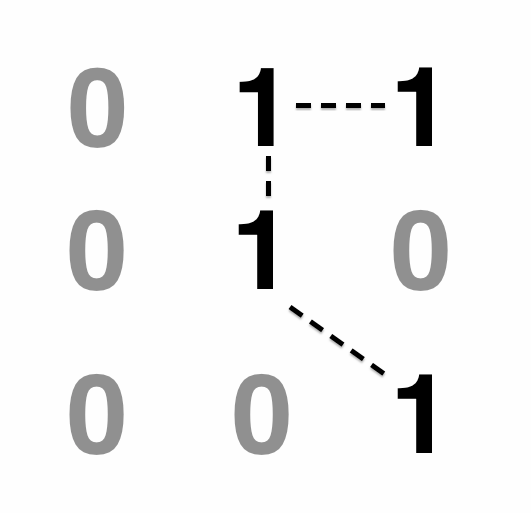
\includegraphics[width = 0.3\textwidth]{./images/m_adjacency}
  \end{minipage}
\end{description}

\subsubsection{Distance measures / Neighbors \buch{p.71}}
For pixels $p,q$  with coordinates $(x,y), (s,t)$
\paragraph{Euclidean}
\begin{equation}
D_e(p,q) = [(x-s)^2 + (y-t)^2]^{\frac{1}{2}}
\end{equation}
\paragraph{City-block}
\begin{equation}
D_4(p,q) = |x-s| + |y-t|
\end{equation}
Pixels with a $D_4 = 1$ are the 4-neighbors of $(x,y)$
\paragraph{Chessboard}
\begin{equation}
D_8(p,q) = max(|x-s|, |y-t|)
\end{equation}
Pixels with a $D_8 = 1$ are the 8-neighbors of $(x,y)$

\subsection{Math tools \buch{p.72}}
\subsubsection{Noise reduction \buch{p.75}}
Image with noise
\begin{equation}
g(x,y) = f(x,y) + \eta(x,y)
\end{equation}
Noise $\eta$ is uncorrelated and has zero average.  Averaging over $K$ different images reduces noise.
\begin{eqnarray}
\bar{g}(x,y)      =& \frac{1}{K} \sum\limits_{i=1}^{K}g_i(x,y) \notag \\
E\{\bar{g}(x,y)\}   =& f(x,y) \\ 
\sigma_{\bar{g}(x,y)}^2 =& \frac{1}{K} \sigma_{\eta(x,y)}^2 \notag
\end{eqnarray}

\subsubsection{Set and Logical Operations \buch{p.80}}
\begin{tabular}{|l|l|l|}
  \hline
  Subset			& $A \subseteq B$						& Every element of A is also in B
  \\ \hline
  Union			& $C = A \cup B$						& C contains all Elements in A, B or both
  \\ \hline
  Intersection	& $D = A \cap B$						& D contains all Elements wich are in A and B
  \\ \hline
  Complement		& $A^c = \{ \omega | \omega \in A\}$	& Set of elements that are not in A
  \\ \hline
  Difference		& $A-B = \{ \omega | \omega \in A, \omega \notin B\} = A \cap B^c$	&
  \\ \hline
\end{tabular}


\subsubsection{Neighborhood operations \buch{p.85}}
Averaging of neighborhood $S_{xy}$
\begin{equation}
g(x,y) = \frac{1}{mn} \sum_{(r,c)\in S_{xy}}f(r,c)
\end{equation}

\subsubsection{Geometric spatial Transformations \buch{p.87}}
\begin{minipage}{0.6\textwidth}
  \[
  (x,y) = T\{(v,w)\} \notag \\
  \]
  \[
  \text{affine transform:} \quad \left[ x~y~1 \right] = [ v~w~q ] \mathbf{T} = [ v~w~1 ] 
  \left[ \begin{array}{ccc}
  t_{11} & t_{12} & 0 \\
  t_{21} & t_{22} & 0 \\
  t_{31} & t_{32} & 1 \end{array} \right]
  \]
\end{minipage}
\begin{minipage}{0.4\textwidth}
  \begin{itemize}
\item Spatial transformation of coordinates
\item Intensity interpolation for transformed pixels
\item See p.88 for examples of $\mathbf{T}$!
\end{itemize}
\end{minipage}

\subsubsection{Image registration \buch{p.89}}
\begin{itemize}
  \item Tries to align several images of the same scheme
  \item Using \textbf{tie points}, whose location are known precisely
\end{itemize}
